\documentclass[12pt]{article}
\usepackage{geometry}
\geometry{a4paper,top=2.5cm,bottom=2.5cm,left=2.3cm,right=2.3cm,heightrounded}
\usepackage{graphicx}
\usepackage{amssymb}
\usepackage{booktabs}
\usepackage[T1]{fontenc}
\usepackage[utf8]{inputenc}
\usepackage{listingsutf8}
\usepackage[italian]{babel}
\usepackage[italian]{varioref}
\usepackage{enumitem}
\usepackage{longtable}
\usepackage{subfig}
\usepackage{fancyhdr}

\title{Progetto di laboratorio \\
\large{Corso di Progettazione Model Driven del Software} \\
\small{https://github.com/gabrielestentella/project}}
\author{Gabriele Stentella}
\date{}

\begin{document}
\maketitle
\section{Descrizione del problema}
\label{sec:descprob}

\subsection{Analisi e specifica dei requisiti}

Viene richiesto di realizzare un applicativo software che aiuti la gestione di attivazione e disattivazione dei tirocini associati alle tesi per i corsi di laurea triennali del Dipartimento di Informatica. Il sistema deve rispettare i seguenti requisiti:
\begin{itemize}
   \item Requisiti funzionali
   \begin{enumerate}
      \item Lo studente deve poter compilare una richiesta di attivazione del tirocinio che può essere interno o esterno
      \item Lo studente deve poter indicare il titolo del tirocinio
      \item Lo studente deve poter indicare i dati anagrafici relativi a se stesso, al relatore, e a eventuali correlatori
      \item Lo studente deve poter indicare la data di inizio e la data di fine del tirocinio
      \item Lo studente deve poter indicare i dati dell'azienda presso cui intende svolgere il tirocinio, in caso di tirocinio esterno
      \item Lo studente deve poter caricare un file pdf contenente l'autocertificazione degli esami sostenuti
      \item Lo studente deve avere la possibilità, direttamente dal modulo della richiesta di attivazione del tirocinio, di navigare verso il \emph{servizio autocertificazioni} per generare il documento richiesto dal sistema
      \item Lo studente deve ricevere una notifica via mail quando la sua richiesta di tirocinio è stata approvata sia dal relatore sia dalla commissione tirocini
      \item Lo studente deve poter controllare lo \emph{stato del tirocinio}, se il tirocinio è in corso deve essere visualizzato il tempo trascorso dalla data di approvazione
      \item Il relatore deve ricevere una notifica via mail quando uno studente compila una richiesta di tirocinio in cui compare come relatore
      \item Il relatore deve poter visualizzare i dati relativi a tutti i tirocini in cui è coinvolto e lo stato di ciascun tirocinio
      \item Il relatore deve poter approvare o rifiutare una richiesta di tirocinio
      \item Il relatore deve poter modificare i dati relativi a un tirocinio già approvato
      \item Il relatore deve poter terminare un tirocinio
      \item La commissione tirocini deve poter visualizzare i dati relativi a tutti i tirocini approvati dai relatori
      \item La commissione tirocini deve poter approvare o rifiutare una richiesta di tirocinio
   \end{enumerate}

   \item Requisiti non funzionali
   \begin{enumerate}
      \item Lo studente deve poter attivare un tirocinio soltanto se ha già superato tutti gli \emph{esami obbligatori} dei primi due anni, oppure ha acquisito almeno 120 \emph{CFU} e deve ancora superare al più un esame fra quelli obbligatori nei primi due anni
      \item Lo studente deve indicare obbligatoriamente uno e un solo relatore, e da zero a due correlatori
      \item Il relatore deve poter terminare un tirocinio solo se si è raggiunta o superata la data di fine del tirocinio
      \item Il tirocinio deve durare almeno 14 settimane e non più di 24
      \item Il relatore è obbligatoriamente un docente dell'ateneo
      \item Se il tirocinio è esterno, deve essere indicato un tutor esterno oltre al relatore accademico
      \item Un docente che fa parte della commissione tirocini non può approvare un tirocinio di cui è relatore accademico
      \item Il correlatore non è da considerarsi un utente del sistema in quanto non può svolgere nessuna operazione sulla richiesta di tirocinio
      \item Se il relatore o la commissione tirocini rifiutano la proposta di tirocinio, lo studente deve ripetere da capo la procedura, i dati della proposta rifiutata non vengono salvati
      \item Requisiti di sviluppo:
      \begin{enumerate}
         \item Il sistema deve essere sviluppato in linguaggio Java
         \item L'interfaccia grafica deve essere sviluppata con JavaFX
         \item I dati persistenti devono essere gestiti con un database relazionale, l'accesso al database deve essere effettuato con la libreria JDBC
      \end{enumerate}
   \end{enumerate}
\end{itemize}

\subsection{Glossario}

\begin{itemize} %DA ORDINARE IN ORDINE ALFABETICO
   \item CFU: Crediti Formativi Universitari, unità di misura dell’impegno richiesto in termini di attività di studio o di apprendimento, un credito corrisponde convenzionalmente a 25 ore di impegno\footnote{fonte: https://www.unimi.it/it/corsi/orientarsi-e-scegliere/il-sistema-universitario}.
   \item esami obbligatori: gli insegnamenti elencati nelle tabelle delle "Attività formative obbligatorie" contenute nel manifesto degli studi reperibile a \texttt{https://apps.unimi.it/} \texttt{files/manifesti/ita\_manifesto\_F68of4\_2024.pdf}.
   \item servizio autocertificazioni: servizio web messo a disposizione dall'ateneo, accessibile dall'url \texttt{https://studente.unimi.it/autocertificati/checkLogin.jsp?0}.
   \item stato del tirocinio\footnote{gli stati del tirocinio sono stati ampliati rispetto alla specifica di progetto}: un tirocinio è in \emph{attesa di approvazione del relatore} (\texttt{attesa1}) dopo che la domanda è stata inviata dallo studente e prima dell'approvazione da parte del relatore; in \emph{attesa di approvazione della commissione} (\texttt{attesa2}) dopo che il relatore lo ha approvato e prima che lo approvi la commissione tirocini; \emph{approvato} dopo l'approvazione da parte della commissione e prima della data di inizio tirocinio; \emph{in corso} (\texttt{in\_corso}) dalla data di inizio tirocinio al momento in cui il relatore termina il tirocinio; \emph{terminato} dopo che il relatore ha terminato il tirocinio.
\end{itemize}

\section{Progettazione del Sistema}
\subsection{Diagramma dei casi d'uso}

La prima versione del diagramma dei casi d'uso prevedeva il caso d'uso "Accedi" collegato a tutti gli utenti del sistema, tuttavia, secondo la notazione UML, se più di un attore è collegato a un caso d'uso vuol dire che per portarlo a completamento serve necessariamente la partecipazione di tutti gli attori, quindi una possibile correzione sarebbe stata quella di creare un attore astratto che fosse una generalizzazione di tutti gli utenti del sistema, ma a fronte delle sostanziali differenze presenti fra i diversi utenti e del fatto che il caso d'uso in questione ha un funzionamento elementare, si è scelto di indicare l'autenticazione dell'utente come precondizione a tutti gli altri casi d'uso ed eliminare il caso d'uso.
Nella seconda versione, oltre ad essere stato eliminato il caso d'uso "Accedi", è stato inserito un nuovo caso d'uso che estende "Compila domanda tirocinio" e consente allo studente di navigare al servizio autocertificazioni.

\begin{figure}[htb!]
   \centering
   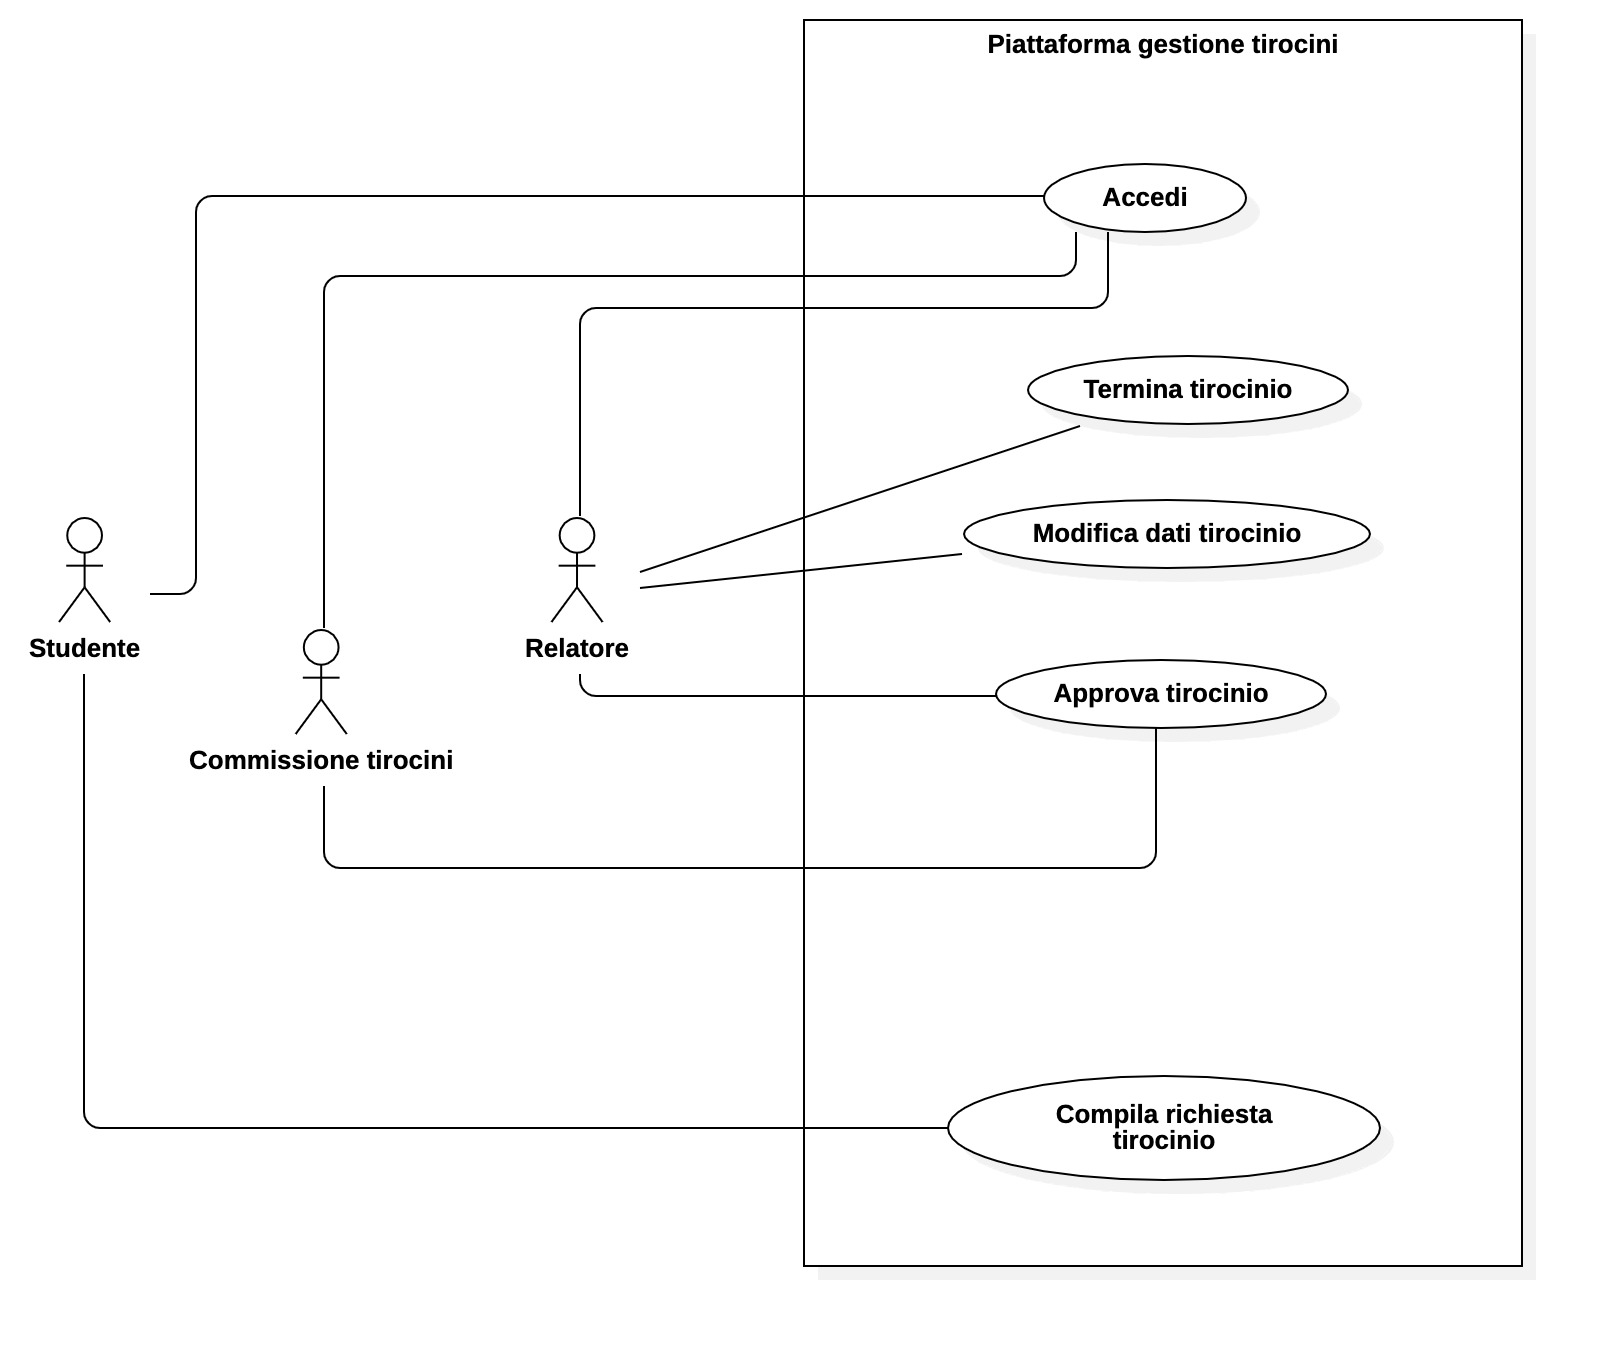
\includegraphics[width=0.7\textwidth]{images/UseCaseDiagram1.jpg}
   \caption*{Prima versione del diagramma dei casi d'uso}
\end{figure}

\begin{figure}[htb!]
   \centering
   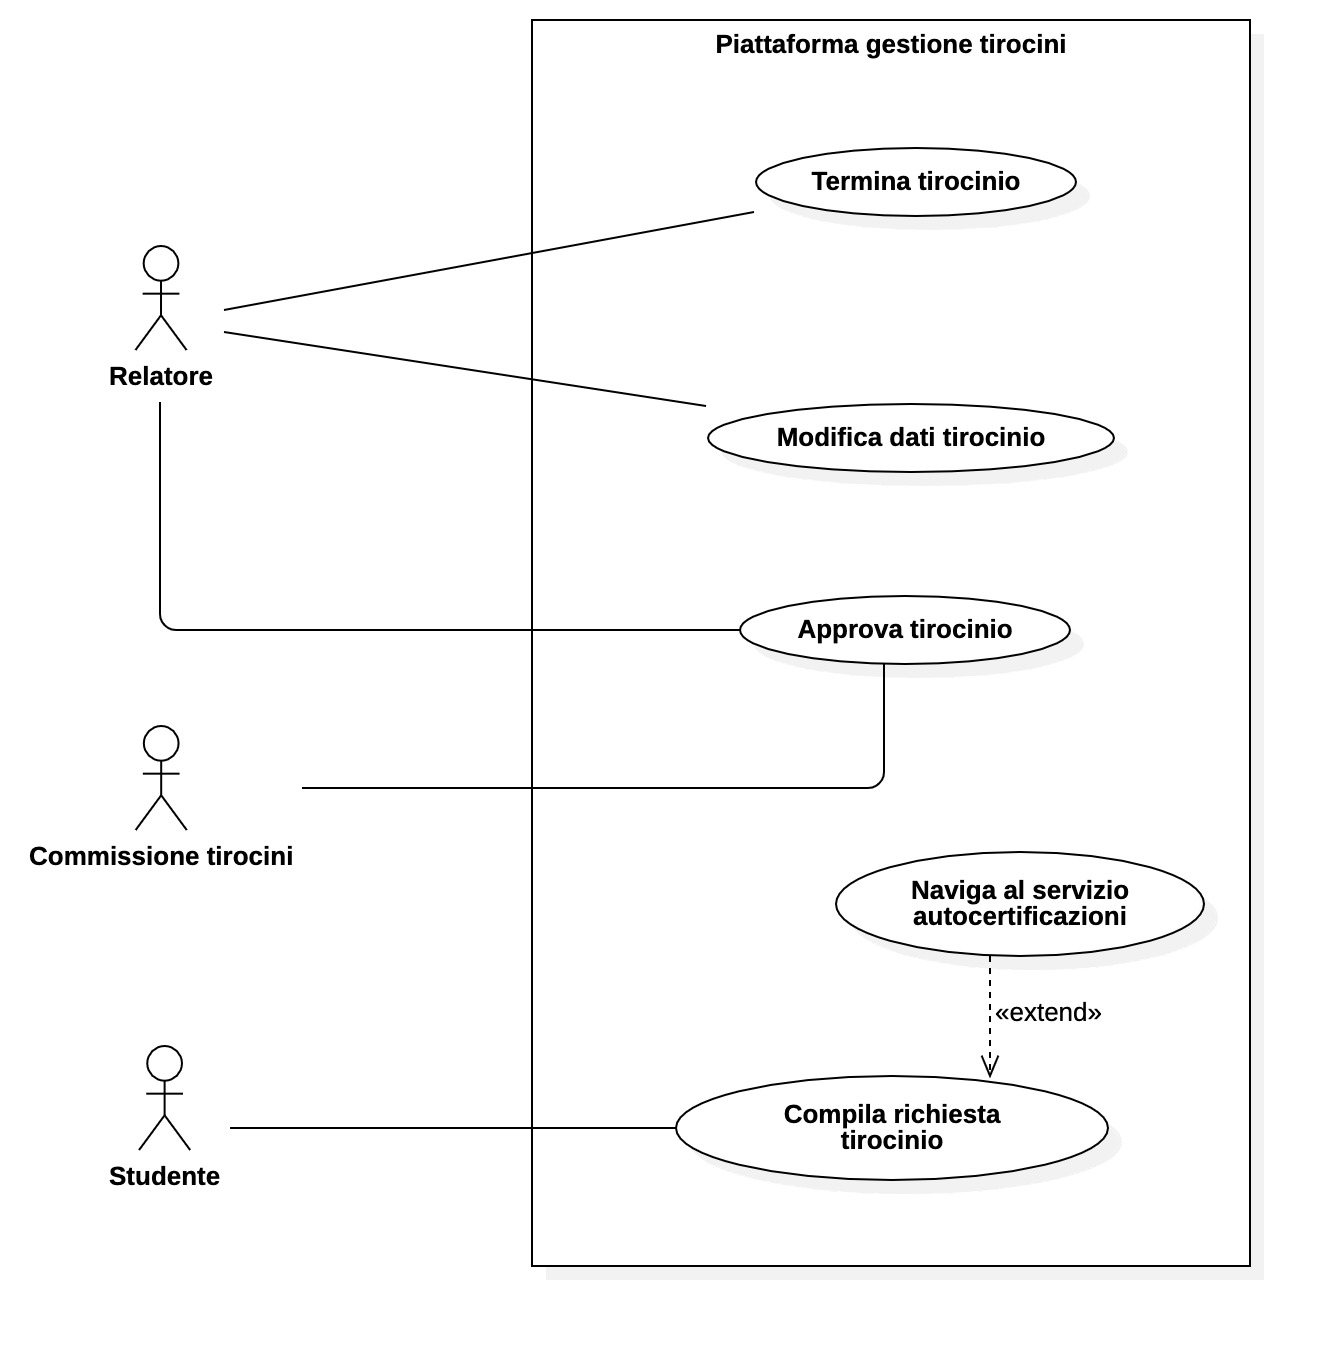
\includegraphics[width=0.7\textwidth]{images/UseCaseDiagram2.jpg}
   \caption*{Seconda versione del diagramma dei casi d'uso}
\end{figure}

\newpage
\subsection{Descrizione degli scenari}

Si riporta di seguito la descrizione degli scenari più significativi per ciascun caso d'uso riportato del diagramma.

 \begin{longtable}{|p{0.35\linewidth} | p{0.6\linewidth}|}
   \hline
   \textbf{Nome} & Compila domanda tirocinio \\ \hline
   \textbf{Scopo} & Lo studente fornisce al sistema la documentazione e i dati necessari all'avvio del tirocinio \\ \hline
   \textbf{Attore} & Studente \\ \hline
   \textbf{Pre-condizioni} & L'utente è autenticato con un account studente \\ \hline
   \textbf{Trigger} & L'utente clicca sul tasto "Nuovo tirocinio" \\ \hline
   \textbf{Descrizione sequenza eventi} &
   \begin{enumerate}[label=(\arabic*)]
      \item Lo studente inserisce il titolo del tirocinio
      \item Lo studente sceglie la tipologia di tirocinio (interno/esterno)
      \item Lo studente inserisce il nome del relatore
      \item Lo studente inserisce la mail di contatto del relatore
      \item Lo studente carica il pdf dell'autocertificazione degli esami sostenuti
      \item Lo studente inserisce la data di inizio tirocinio
      \item Lo studente inserisce la data di fine tirocinio
      \item Lo studente invia la richiesta
      \item Il sistema chiede conferma dei dati inseriti
      \item Lo studente conferma i dati
      \item Il sistema visualizza una schermata di conferma
      \item Il sistema invia una mail di notifica allo studente e al relatore
      \item Il sistema scrive i dati della richiesta di tirocinio nel database
   \end{enumerate} \\ \hline
   \textbf{Alternative} &
   \begin{enumerate}[label=(\arabic*')]
      \setcounter{enumi}{4}
      \item Lo studente inserisce il nome del correlatore
      \item Lo studente inserisce la mail di contatto del correlatore
      \item Il processo riprende da (5') se è presente un correlatore aggiuntivo, altrimenti riprende da (5)
   \end{enumerate}
   ––––––––––––––––––––––––––––––––––––––––––––––-
   \begin{enumerate}[label=(\arabic*')]
      \setcounter{enumi}{4}
      \item Lo studente clicca sul tasto "Servizio autocertificazioni"
      \item Lo studente utilizza il servizio per generare il documento richiesto
      \item Il processo riprende da (5)
   \end{enumerate}
   \\ \hline
   \textbf{Post-condizioni} & La richiesta di tirocinio viene registrata nel database dedicato \\ \hline
 \end{longtable}

 \begin{longtable}{|p{0.35\linewidth} | p{0.6\linewidth}|}
 \hline
 \textbf{Nome} & Approva tirocinio \\ \hline
 \textbf{Scopo} & L'utente approva una proposta di tirocinio effettuata da uno studente  \\ \hline
  \textbf{Attore} & Relatore, Commissione tirocini \\ \hline
  \textbf{Pre-condizioni} & L'utente è autenticato con un account relatore o commissione tirocini, esiste almeno un tirocinio che si trova in uno dei due stati di attesa dell'approvazione \\ \hline
  \textbf{Trigger} & L'utente seleziona una richiesta di tirocinio che vede nella propria homepage \\ \hline
  \textbf{Descrizione sequenza eventi} &
  \begin{enumerate}[label=(\arabic*)]
      \item L'utente visualizza i dati relativi alla richiesta di tirocinio che ha selezionato
      \item L'utente clicca su "Approva tirocinio"
      \item Il sistema richiede di confermare l'azione
      \item L'utente conferma
      \item Il sistema torna all'homepage
      \item Il sistema riporta l'approvazione nel database
      \item Il sistema controlla se il tirocinio è stato approvato sia dal Relatore sia dalla Commissione tirocini, in caso positivo invia una mail di notifica allo studente
  \end{enumerate} \\ \hline
  \textbf{Alternativa} &
  \begin{enumerate}[label=(\arabic*')]
      \setcounter{enumi}{1}
      \item L'utente clicca su "Rifiuta tirocinio"
      \item (3', 4' e 5') uguali alla sequenza principale
      \setcounter{enumi}{5}
      \item Il sistema riporta il rifiuto nel database
      \item Il sistema invia una mail di notifica allo studente
  \end{enumerate} \\ \hline
  \textbf{Post-condizioni} & La richiesta di tirocinio viene marcata come approvata o rifiutata dall'utente nel database dedicato \\ \hline
 \end{longtable}

 \begin{longtable}{|p{0.35\linewidth} | p{0.6\linewidth}|}
 \hline
 \textbf{Nome} & Modifica dati tirocinio \\ \hline
 \textbf{Scopo} & Il relatore può modificare i dati relativi a un tirocinio approvato \\ \hline
  \textbf{Attore} & Relatore \\ \hline
  \textbf{Pre-condizioni} & L'utente è autenticato con un account relatore \\ \hline
  \textbf{Trigger} & L'utente seleziona una richiesta di tirocinio che vede nella propria homepage \\ \hline
  \textbf{Descrizione sequenza eventi} &
  \begin{enumerate}[label=(\arabic*)]
      \item L'utente effettua una modifica sui dati del tirocinio che ha selezionato
      \item L'utente conferma le modifiche
      \item Il sistema torna all'homepage
      \item Il sistema riporta le modifiche nel database dedicato
  \end{enumerate} \\ \hline
  \textbf{Post-condizioni} & I dati relativi a un tirocinio sono modificati nel database \\ \hline
 \end{longtable}

 \begin{longtable}{|p{0.35\linewidth} | p{0.6\linewidth}|}
 \hline
 \textbf{Nome} & Termina tirocinio \\ \hline
 \textbf{Scopo} & Il relatore può marcare un tirocinio come terminato  \\ \hline
  \textbf{Attore} & Relatore \\ \hline
  \textbf{Pre-condizioni} & L'utente è autenticato con un account relatore, la data indicata come fine del tirocinio è pari o inferiore a quella in avviene questo caso d'uso \\ \hline
  \textbf{Trigger} & L'utente seleziona una richiesta di tirocinio che vede nella propria homepage \\ \hline
  \textbf{Descrizione sequenza eventi} &
  \begin{enumerate}[label=(\arabic*)]
      \item L'utente clicca sul tasto "Termina tirocinio"
      \item Il sistema richiede di confermare la chiusura del tirocino
      \item L'utente conferma
      \item Il sistema torna all'homepage
      \item Il sistema marca il tirocinio come terminato nel database
  \end{enumerate} \\ \hline
  \textbf{Post-condizioni} & Il tirocinio è marcato come terminato nel database \\ \hline
 \end{longtable}


\subsection{Diagramma delle classi}
\label{sec:claprogetto}

Si riporta il diagramma delle classi di progetto. Le classi \emph{Docente} e \emph{Studente}, avendo molti attributi in comune, sono state legate con una relazione di ereditarietà alla classe astratta \emph{UtenteUniversità}, inoltre il fatto che la \emph{CommissioneTirocini} è composta da più docenti, è riportato del diagramma con l'utilizzo di una relazione di aggregazione (in quanto l'esistenza di un'istanza di \emph{Docente} non è condizionata alla sua appartenenza alla commissione). La classe centrale è \emph{Tirocinio}, contiene tutti gli attributi necessari (requisiti 1 — 6) alla memorizzazione di una richiesta di tirocinio e a gestire il suo stato, e tutti i metodi legati alla variazione di stato.

\begin{figure}[htb!]
   \centering
   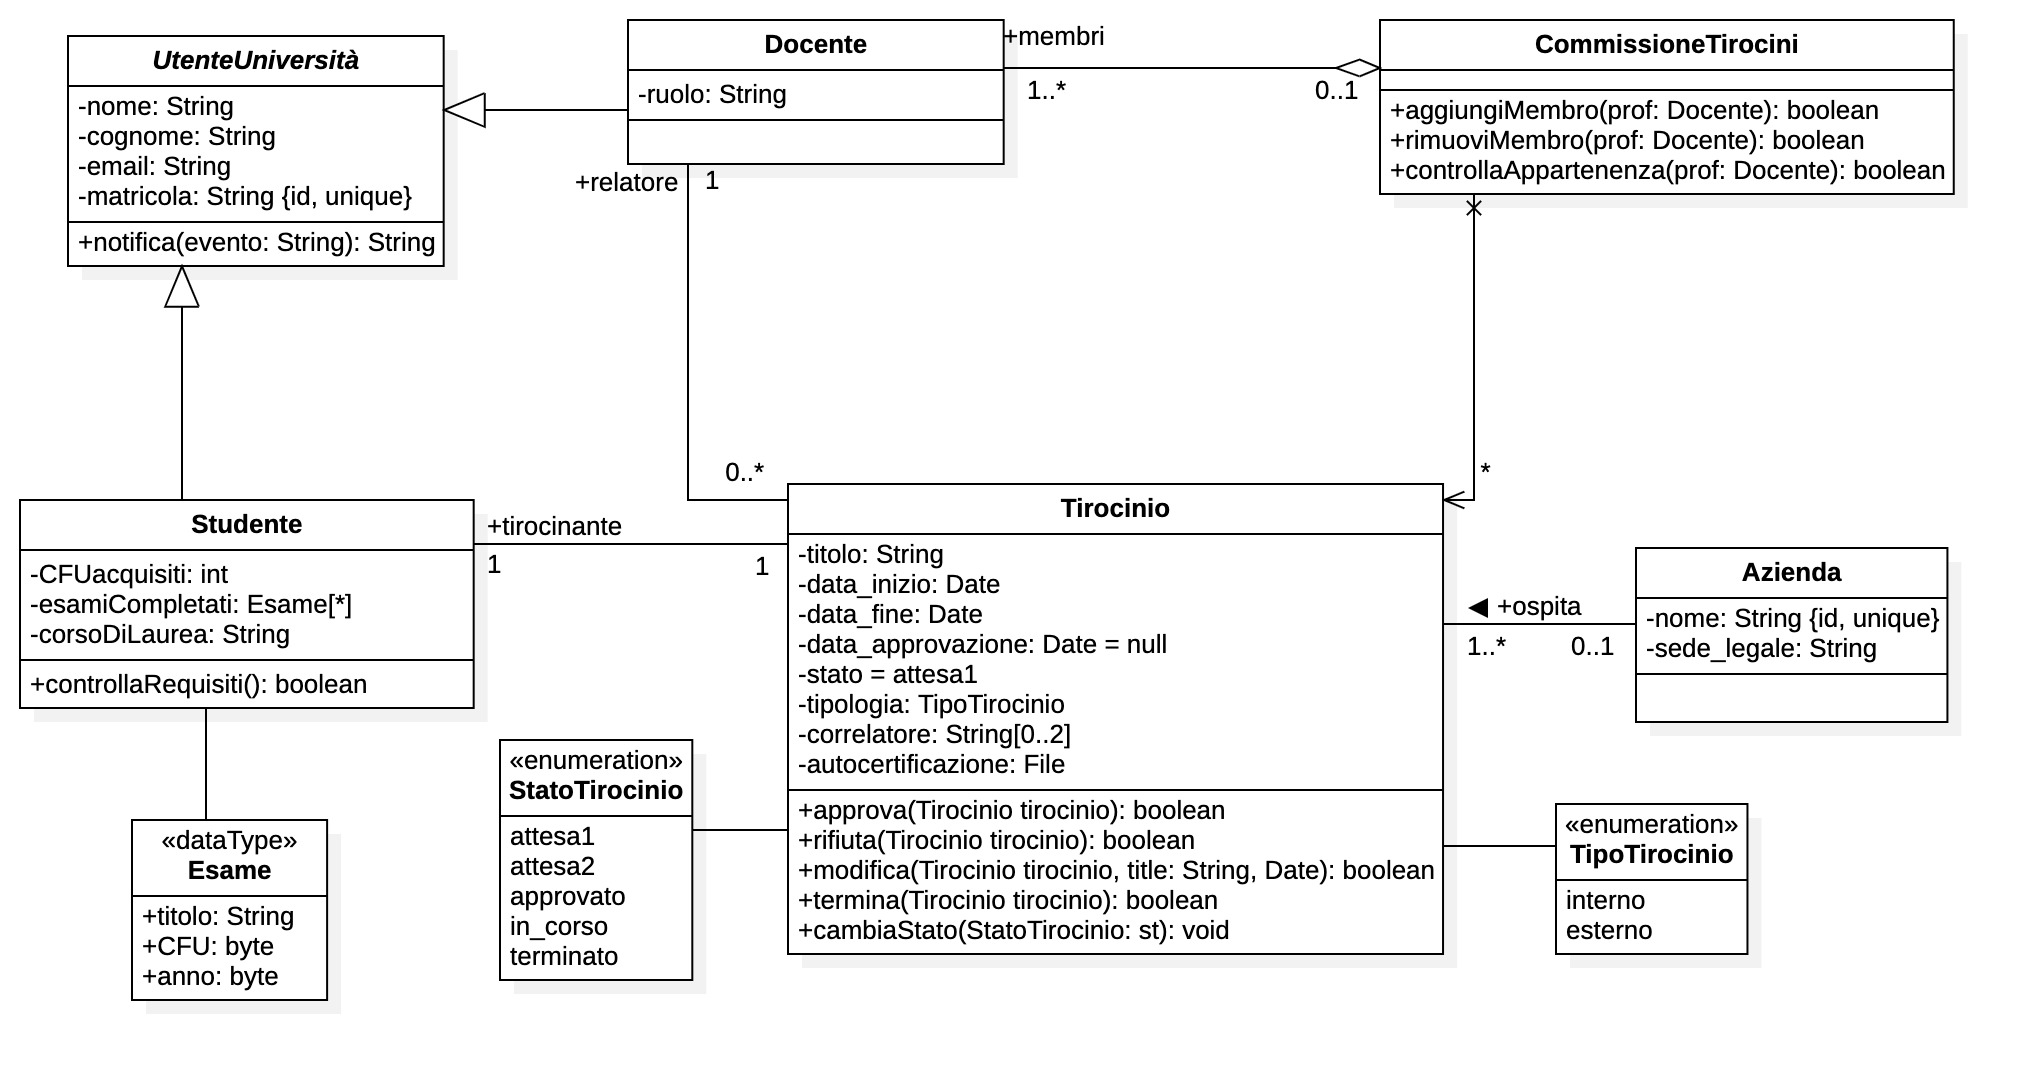
\includegraphics[width=\textwidth]{images/ClassDiagramProgetto.jpg}
   \caption*{Diagramma delle classi di progetto}
\end{figure}


\subsection{Diagrammi di sequenza}

Per ogni caso d'uso, viene riportato il rispettivo diagramma di sequenza, le sequenze più significative sono legate ai casi d'uso \emph{Compila richiesta tirocinio} e \emph{Approva tirocinio}.

\begin{figure}[htb!]
   \centering
   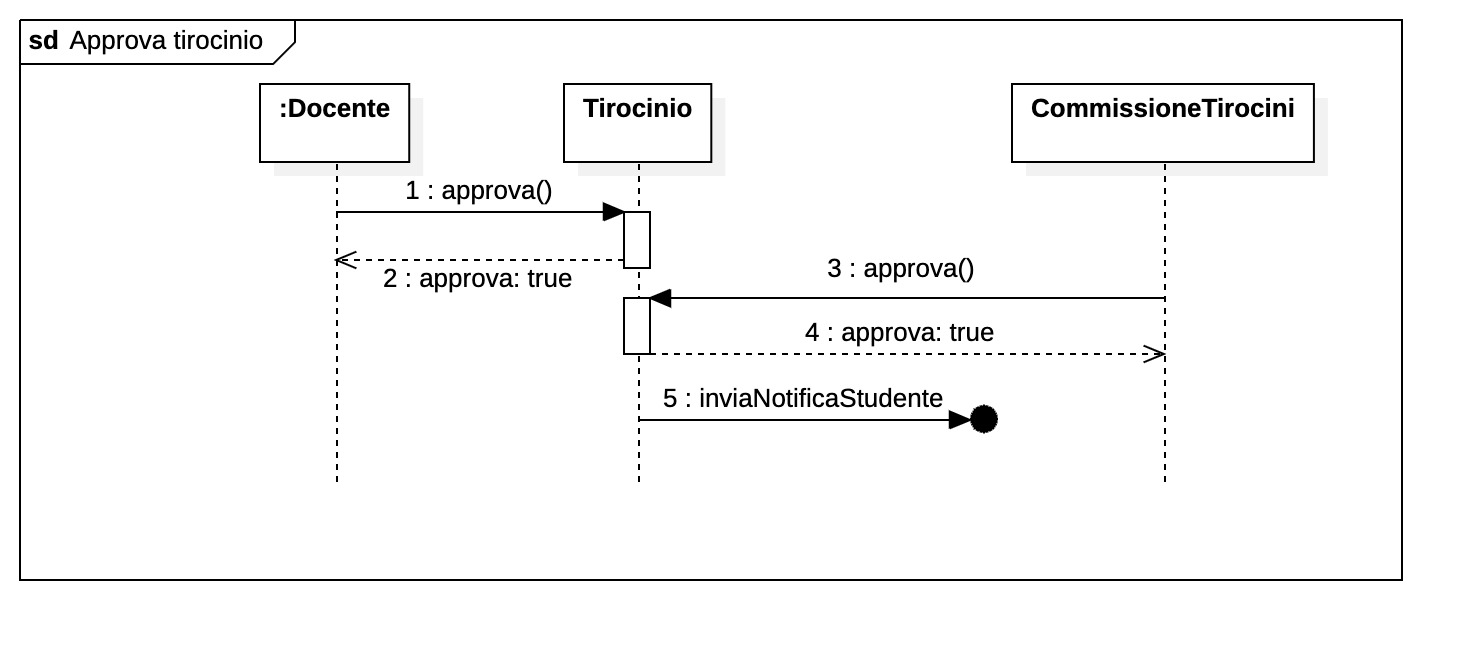
\includegraphics[width=\textwidth]{images/Approva tirocinio.jpg}
   \caption*{Diagramma di sequenza del caso d'uso \emph{Approva tirocinio}}
\end{figure}

\begin{figure}[htb!]
   \centering
   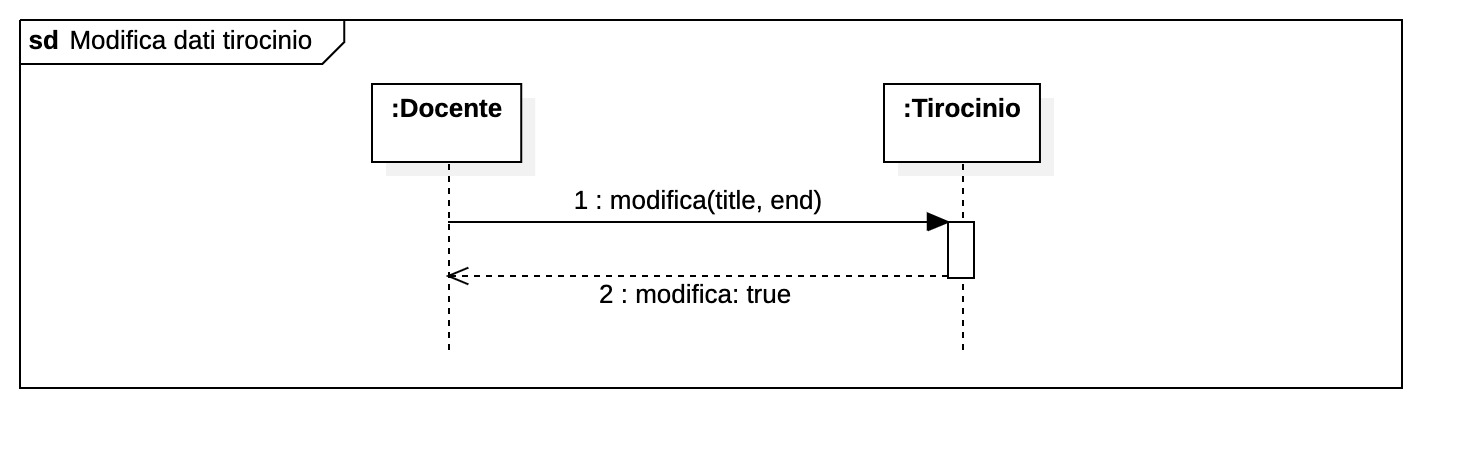
\includegraphics[width=\textwidth]{images/Modifica dati tirocinio.jpg}
   \caption*{Diagramma di sequenza del caso d'uso \emph{Modifica dati tirocinio}}
\end{figure}

\begin{figure}[htb!]
   \centering
   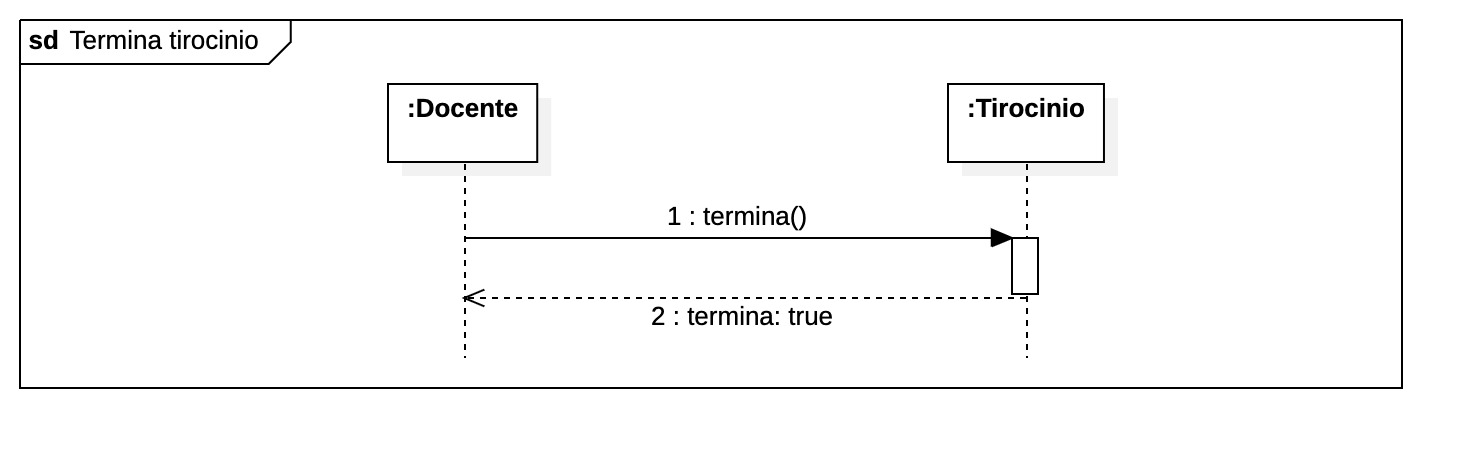
\includegraphics[width=\textwidth]{images/Termina tirocinio.jpg}
   \caption*{Diagramma di sequenza del caso d'uso \emph{Termina tirocinio}}
\end{figure}

\begin{figure}[htb!]
   \centering
   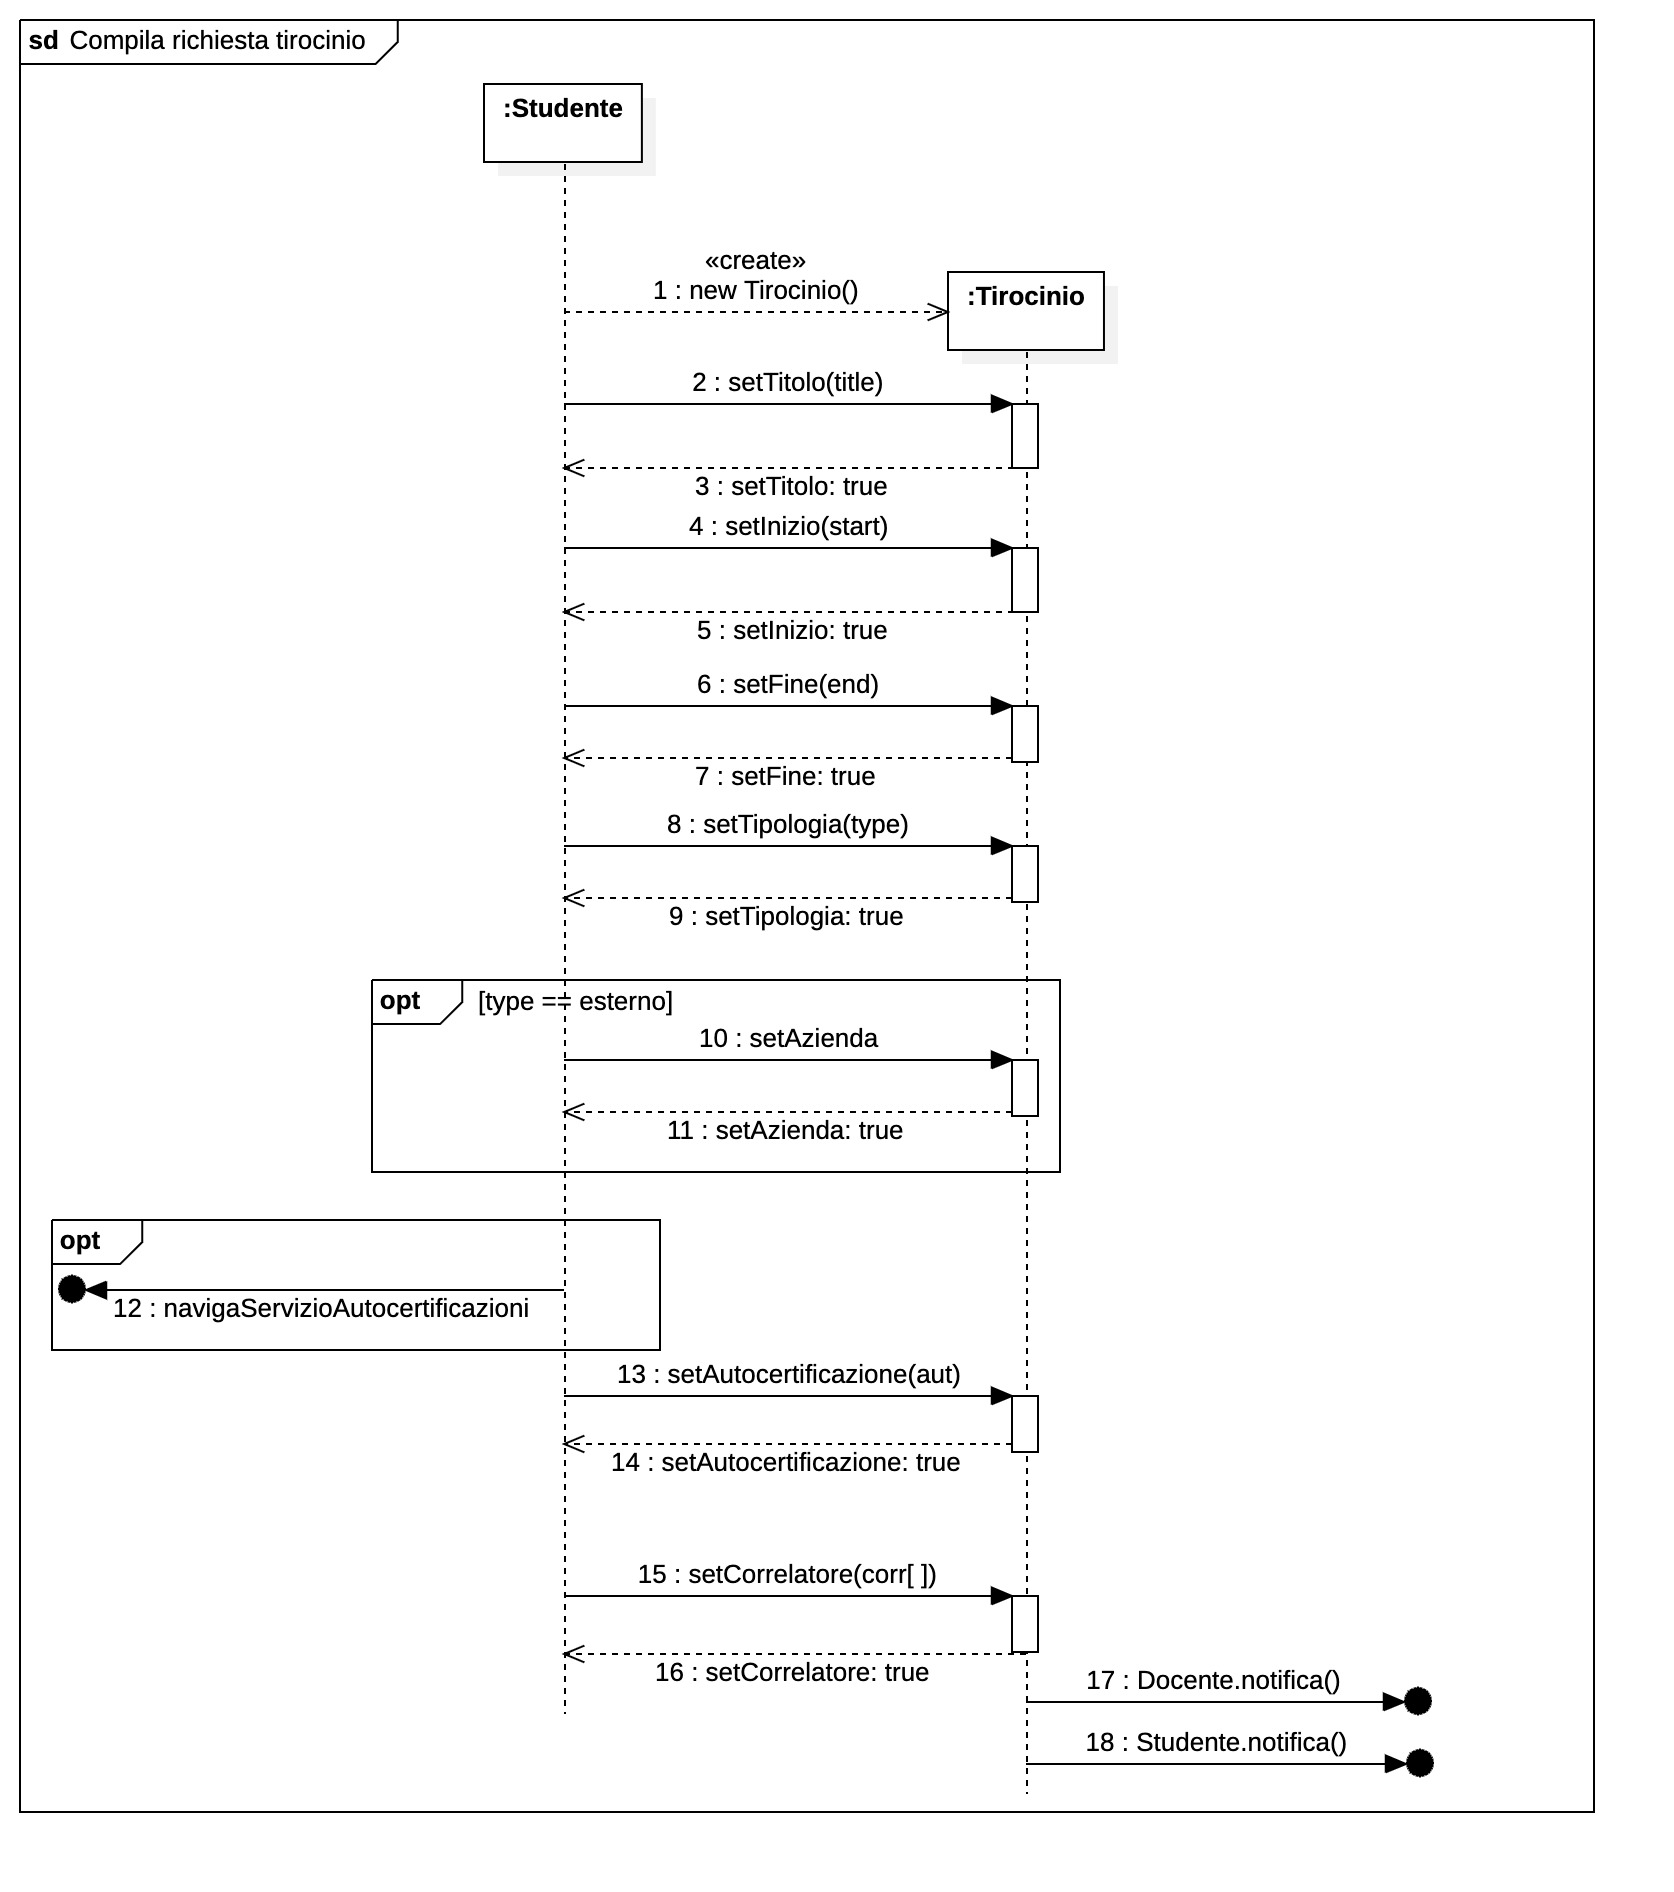
\includegraphics[width=\textwidth]{images/Compila richiesta tirocinio.jpg}
   \caption*{Diagramma di sequenza del caso d'uso \emph{Compila richiesta tirocinio}}
\end{figure}

\newpage


\subsection{Diagrammi delle attività}

Dal momento che il programma è completamente incentrato sulla gestione del tirocinio, il suo intero funzionamento è riassumibile in un'unica sequenza. Il ciclo di vita di un tirocinio comincia con la compilazione di una richiesta, poi evolve passando dai vari stati in base alle azioni compiute da \emph{Docente} e \emph{Commissione tirocini}. I dati che sono da memorizzare in maniera persistente sono inseriti in nodi \emph{<<datastore>>} (si veda il diagramma delle classi di programma, sezione \ref{sec:claprogramma}, per i dettagli relativi alla gestione del database).

\begin{figure}[h!]
   \centering
   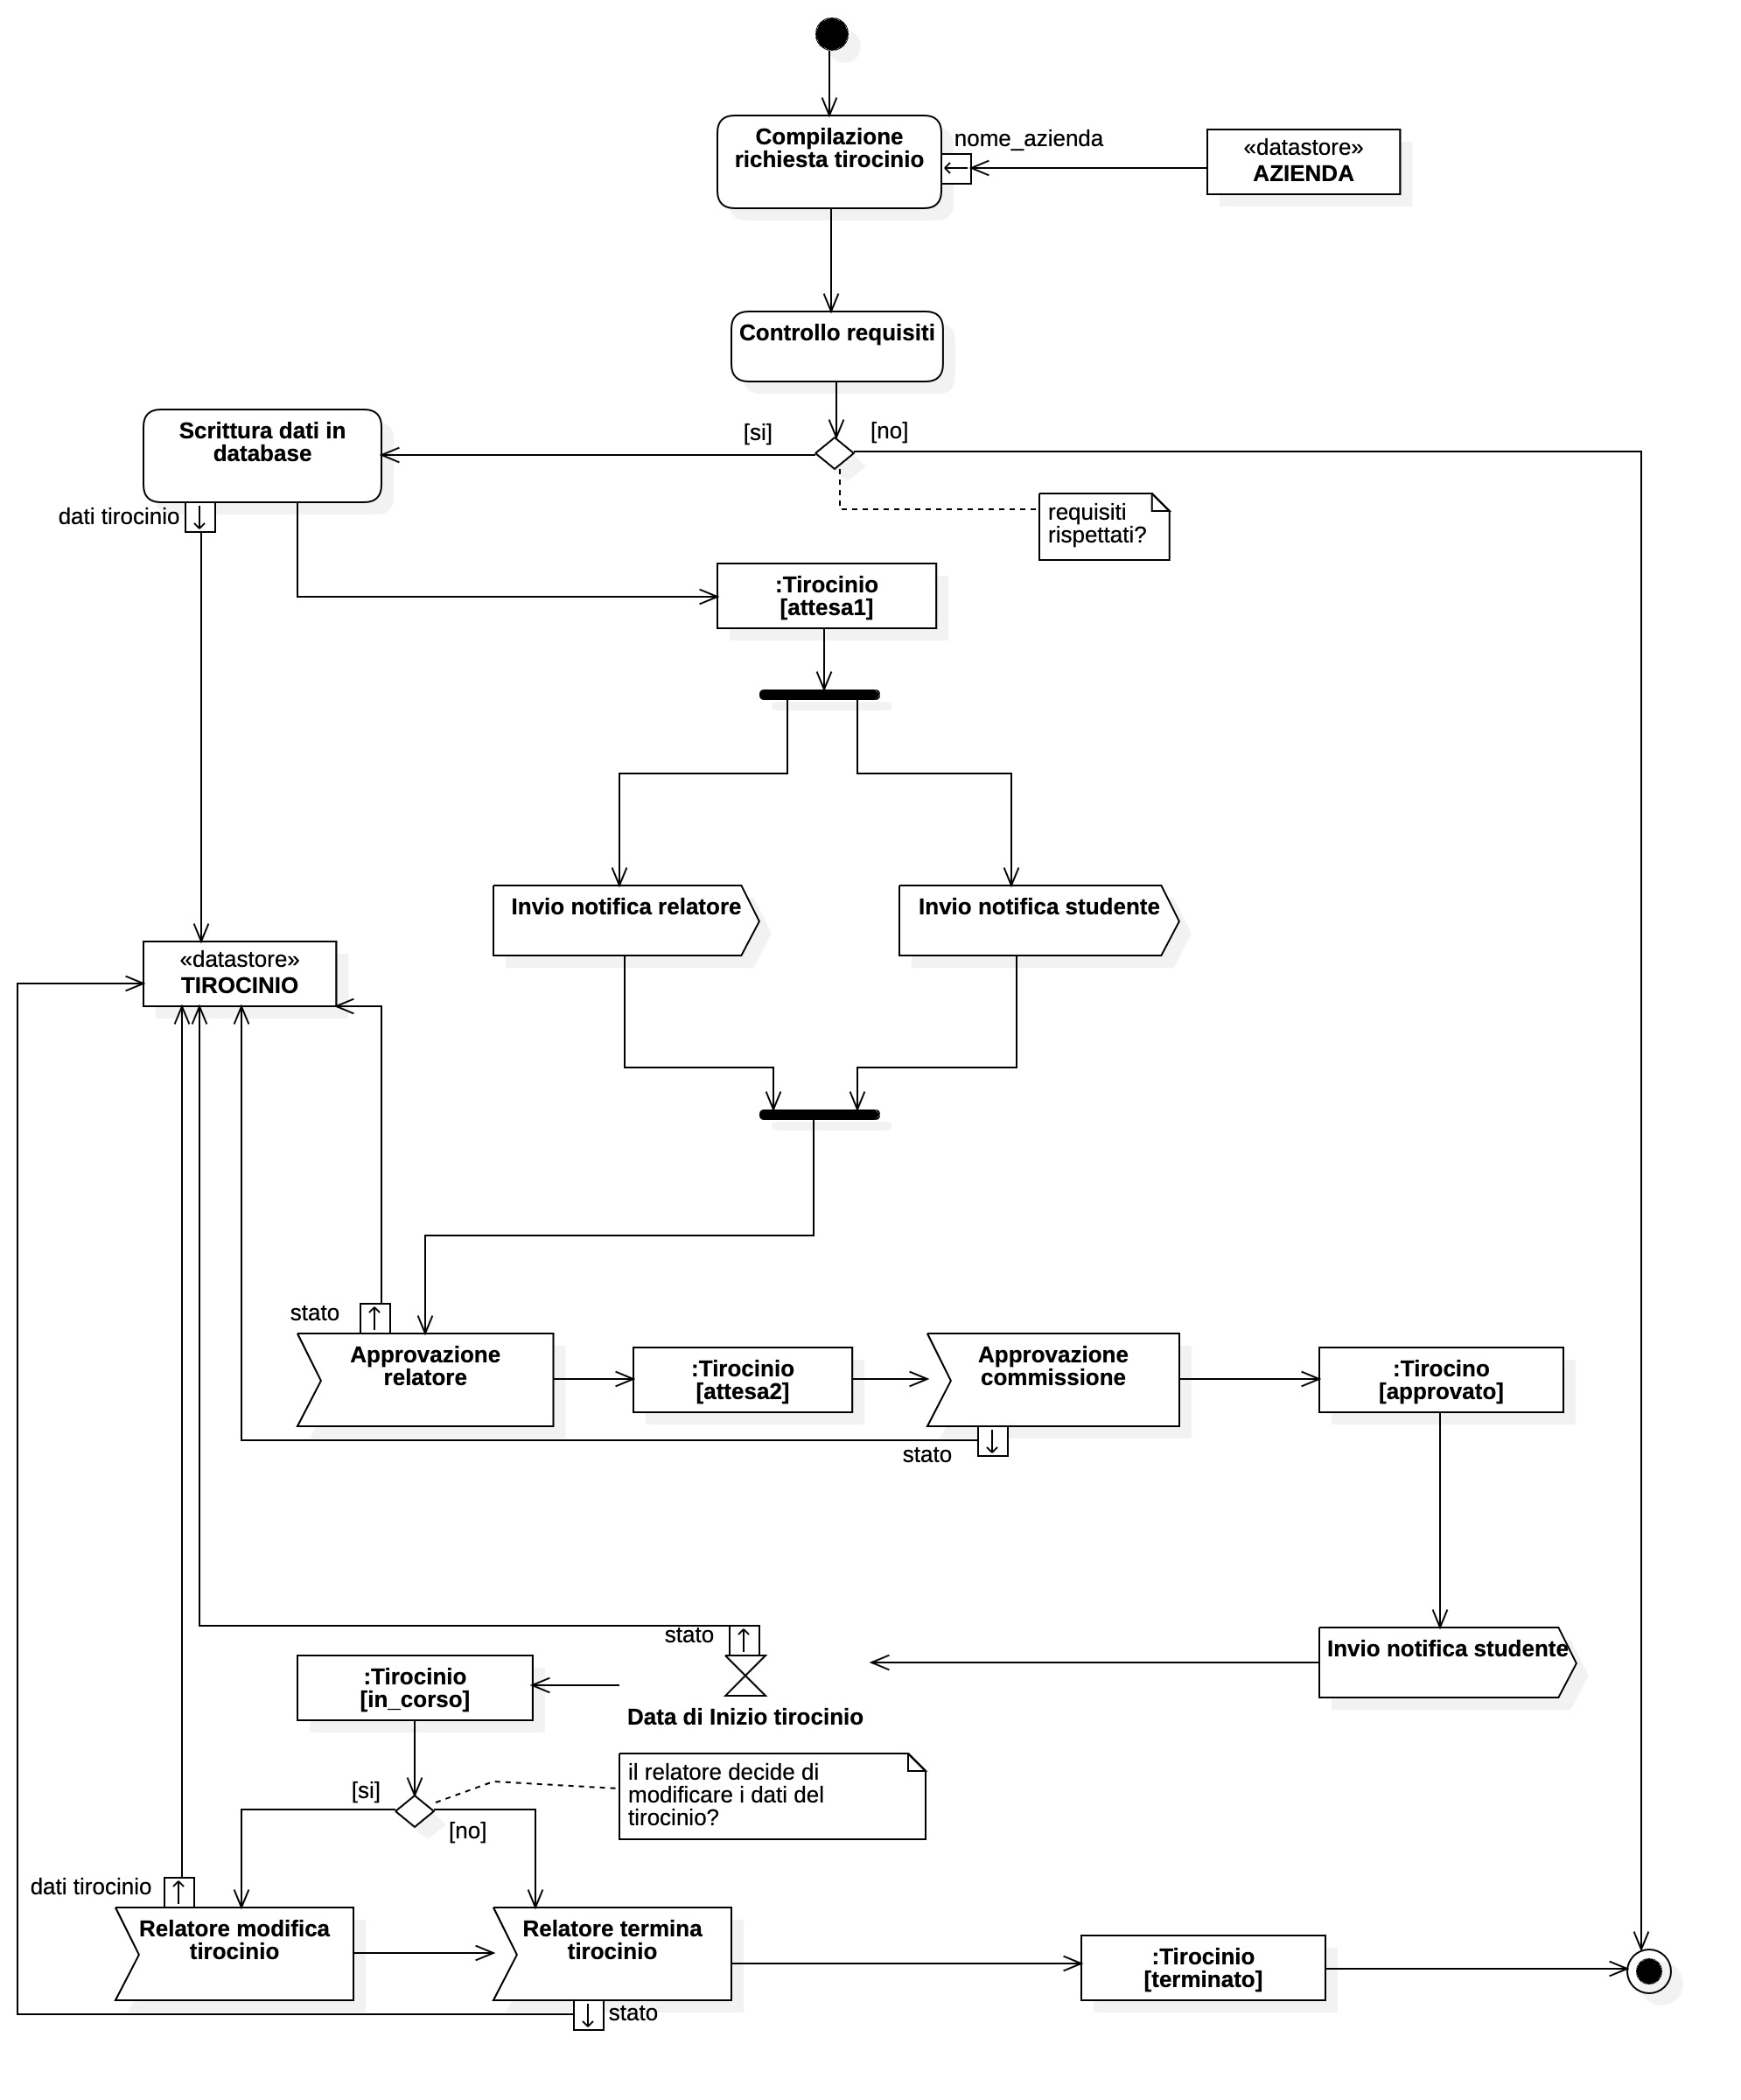
\includegraphics[width=\textwidth]{images/ActivityDiagram1.jpg}
   \caption*{Diagramma di attività}
\end{figure}

\newpage


\subsection{Macchine di stato}
\label{subsec:state}

L'unica entità dell'applicativo che è caratterizzata da stati rilevanti per lo sviluppo del software è il Tirocinio. Come spiegato nel glossario (sezione \ref{sec:descprob}), il Tirocinio si trova nello stato \texttt{attesa1} appena viene inserito nel sistema, poi passa nello stato \texttt{attesa2} quando viene approvato dal relatore, quando viene approvato anche dalla commissione tirocini passa nello stato \texttt{approvato}, a partire dalla data di inizio indicata nella richiesta (evento temporale) il Tirocinio si trova nello stato \texttt{in\_corso}, quando il relatore decide di terminare il Tirocinio, lo stato passa a \texttt{terminato}. Sia quando il Tirocinio si trova nello stato \texttt{approvato}, sia quando è \texttt{in\_corso}, il relatore può effettuare delle modifiche ai dati, questa operazione non modifica lo stato del tirocinio. Se il relatore o la commissione tirocini rifiutano la proposta di tirocinio, l'oggetto Tirocinio viene distrutto.
Si riporta la macchina di stato UML:

\begin{figure}[h!]
   \centering
   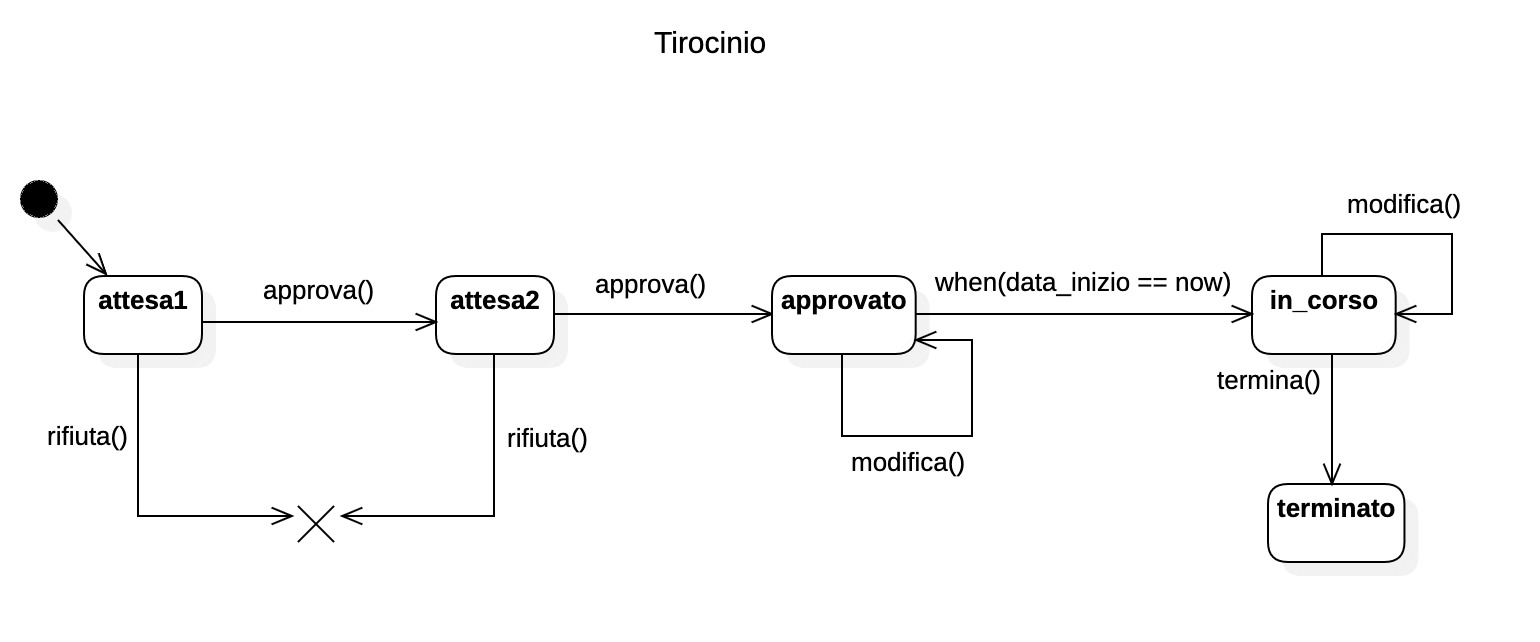
\includegraphics[width=\textwidth]{images/StatechartDiagram1.jpg}
   \caption*{Diagramma della macchina di stato}
\end{figure}

\section{Dettagli architetturali del Sistema}
\subsection{Diagramma delle classi di programma}
\label{sec:claprogramma}

Rispetto al diagramma delle classi di progetto (\ref{sec:claprogetto}), questo diagramma è realizzato con l'intento di essere il più possibile vicino al codice, quindi sono stati aggiunti i metodi \textit{getter} e \textit{setter} e le classi che implementano la logica di accesso al database. Sono state aggiunte le classi necessarie ad implementare i design pattern (vedere la sezione seguente) e tutte le classi presenti nel diagramma sono state divise in package.

\begin{figure}[htb!]
   \centering
   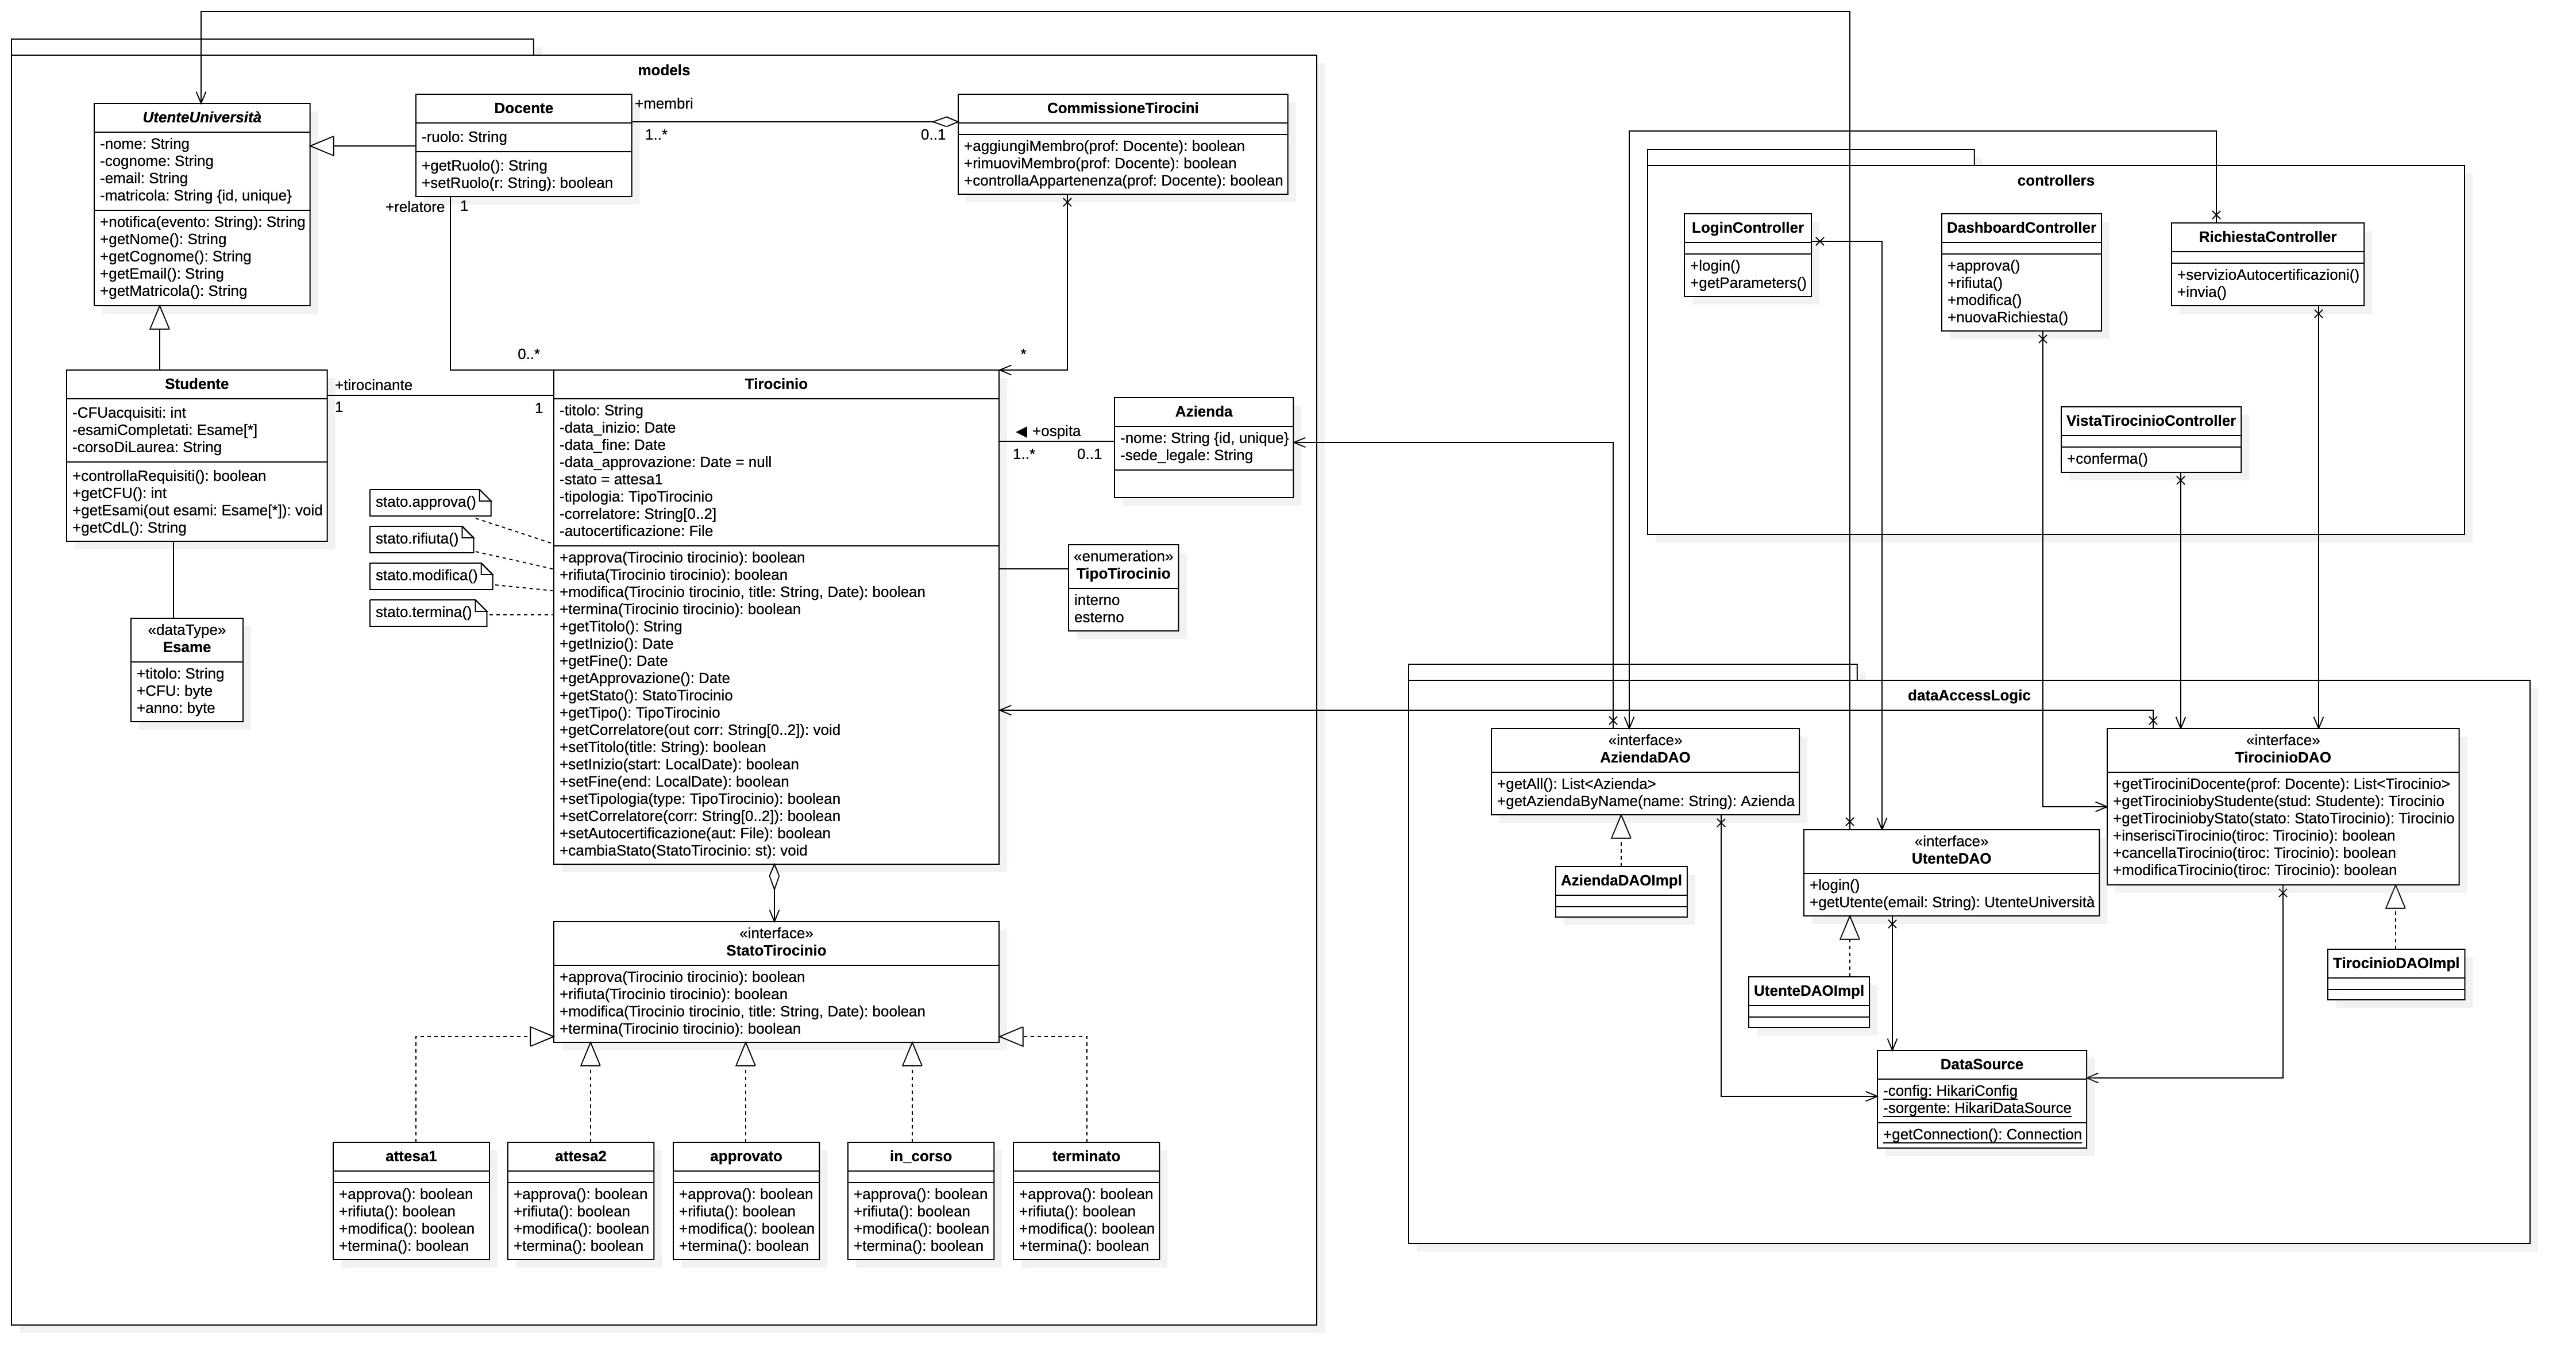
\includegraphics[width=\textwidth]{images/ClassDiagramProgramma.jpg}
   \caption*{Diagramma delle classi di programma}
\end{figure}

\subsubsection{Pattern architetturali}
\begin{itemize}
   \item Model View Controller: l'intero progetto è stato pensato seguendo il pattern MVC, infatti il codice è organizzato in tre packages\footnote{La logica di accesso al database è in un package separato}, uno per i modelli, uno per i controllers e uno per le viste, che sono file FXML. Questo pattern consente di dividere le classi che rappresentano il dominio, ovvero i modelli, dall'interfaccia grafica e dalle classi che servono a manipolarla.
   \item Data Access Object: l'accesso al database è gestito attraverso il pattern DAO, che prevede l'utilizzo di un'interfaccia e una classe che implementa tale interfaccia per creare un oggetto che consente di trasferire i dati da e verso il database.
   \item State: la classe Tirocinio è stateful e il suo stato è gestito con il pattern State, quindi la classe è in relazione con un'interfaccia che consente di gestire ogni possibile input, poi ogni stato implementa l'interfaccia e realizza i cambiamenti di stato in base all'input ricevuto. Rispetto al diagramma delle classi di progetto, in cui lo stato era gestito con un tipo enumerativo, per implementare il pattern ogni stato è una classe.
\end{itemize}
\textbf{Nota:} la connessione al database \emph{non} è stata implementata utilizzando il pattern singleton, ma sfruttando un meccanismo di connection pooling, implementato con Hikari. La scelta si deve alle performance migliori offerte dal pooling e dal fatto che il singleton può non essere thread safe.

\newpage


\subsection{Diagramma dei componenti}

Il programma è rappresentato da un unico componente centrale che contiene i componenti models, views, controllers e dataAccessLogic, e utilizza i servizi offerti da componenti esterni per connettersi al database, per inviare le email di notifica e per il logging. Il sistema di logging è implementato con il framework Apache Log4j, scelto in quanto open source e largamente adottato.

\begin{figure}[h!]
   \centering
   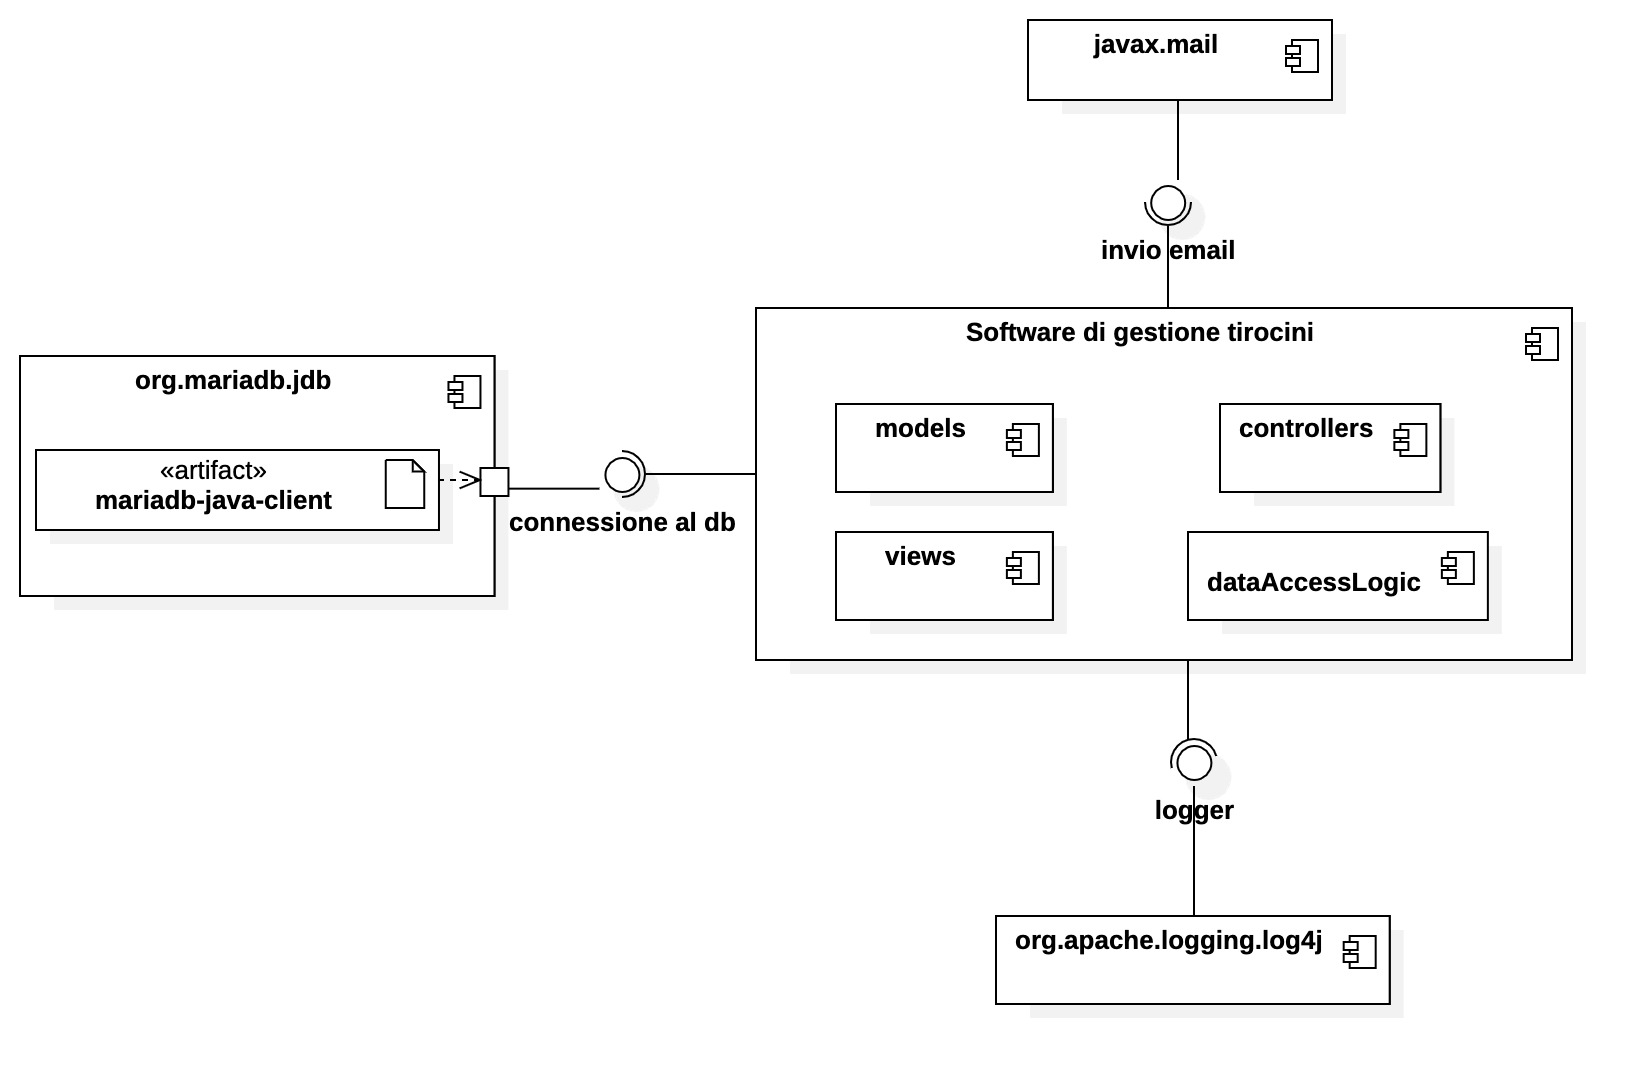
\includegraphics[width=\textwidth]{images/ComponentDiagram1.jpg}
   \caption*{Diagramma dei componenti}
\end{figure}

\newpage


\subsection{Diagramma di deployment}

Tutto l'applicativo software viene eseguito sulla macchina dell'utente, anche il database è gestito localmente. Per inviare le email e generare le autocertificazioni, il pc utente si interfaccia con i server dedicati di unimi. La comunicazione con il database avviene utilizzando JDBC, con il server mail è tramite il protocollo SMTP, con il servizio autocertificazioni è tramite il protocollo HTTPS.

\begin{figure}[h!]
   \centering
   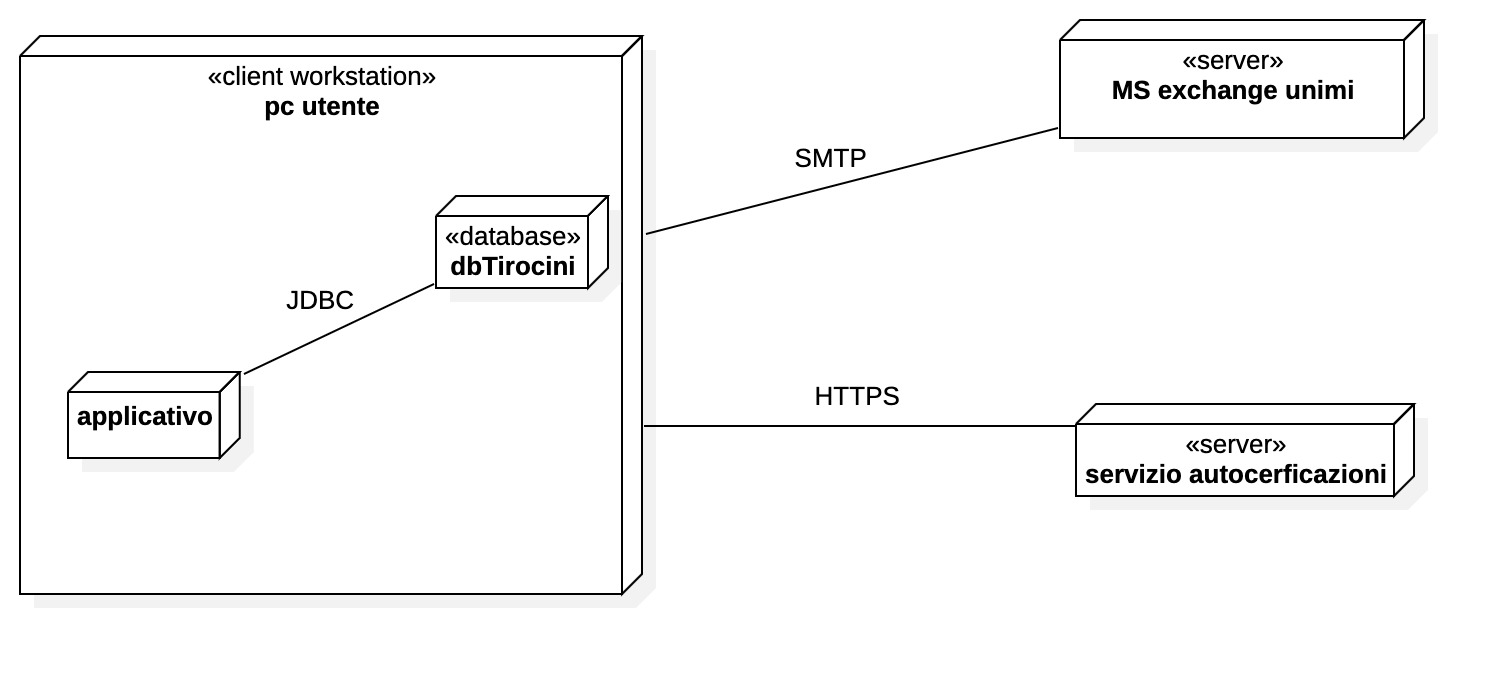
\includegraphics[width=\textwidth]{images/DeploymentDiagram1.jpg}
   \caption*{Diagramma di deployment}
\end{figure}

\section{Dettagli implementativi}

\subsection{Java e JavaFX}

La versione di Java utilizzata è Java SE 8 (SDK Oracle OpenJDK 21.0.1), JavaFX API versione 21.


\subsection{Software manager}

Il progetto è gestito con il tool Apache Maven\footnote{https://maven.apache.org}, che consente di gestire le dipendenze delle librerie esterne e implementare i plugin necessari alla compilazione e alla distribuzione del software. La configurazione di Maven è basata sul project object model (POM), nello specifico tutte le informazioni di configurazione, le dipendenze e i plugin sono riportati in un file in eXtensible Markup Language.


\subsection{Database}

Il database relazionale è gestito con il DBMS MariaDB\footnote{https://mariadb.com}, il software si interfaccia al DBMS usando l'API JDBC MariaDB Connector/J, versione 3.3.2.

Il database è composto da 4 tabelle:
\begin{enumerate}
   \item \textit{Utente} contiene email, password e tipo;
   \item \textit{Studente} contiene tutti gli attributi della classe Studente;
   \item \textit{Docente} contiene tutti gli attributi della classe Docente;
   \item \textit{Azienda} contiene tutti gli attributi della classe Azienda.
\end{enumerate}


\subsection{Gestione delle password}

Le password sono memorizzate nel database come un hash che viene calcolato utilizzando l'algoritmo bcrypt implementato da BCryptPasswordEncoder di Spring security. Il matching della password è effettuato sempre tramite BCryptPasswordEncoder, è volutamente lento per rendere più difficili gli attacchi, quindi il login impiega circa 5 secondi.


\subsection{Vincoli}

I vincoli di seguito riportati in Object Constraint Language (OCL) sono scritti in Java Modeling Language (JML) direttamente nel codice.

Dal requisito non funzionale n°2: "lo studente deve indicare \emph{obbligatoriamente} uno e un solo relatore [...]".
\begin{verbatim}
{ context Tirocinio
  inv: self.relatore <> null }
\end{verbatim}

Dal requisito non funzionale n°6: "se il tirocinio è esterno, deve essere indicato un tutor esterno oltre al relatore accademico".
\begin{verbatim}
{ context Tirocinio
  inv: self.tipologia == #esterno implies self.correlatore.length >= 1 }
\end{verbatim}

I vincoli di seguito servono per accertarsi che i metodi che cambiano lo stato eseguano i passaggi secondo la macchina di stato riportata nella sezione \ref{subsec:state}.
\begin{verbatim}
{ context Tirocinio::approva():boolean
  pre: self.oclInState(attesa1) or self.oclInState(attesa2)
  post: self@pre.oclInState(attesa1) implies self.oclInstate(attesa2)
        and self@pre.oclInState(attesa2) implies self.oclInstate(approvato) }
\end{verbatim}

\begin{verbatim}
{ context Tirocinio::rifiuta():boolean
  pre: self.oclInState(attesa1) or self.oclInState(attesa2)
  post: self.stato == null }
\end{verbatim}

\begin{verbatim}
{ context Tirocinio::modifica():boolean
  pre: self.oclInState(approvato) or self.oclInState(in_corso)
  post: self@pre.oclInState(approvato) implies self.oclInState(approvato)
        and self.oclInState(in_corso) implies self.oclInState(in_corso) }
\end{verbatim}

\begin{verbatim}
{ context Tirocinio::termina():boolean
  pre: self.oclInState(in_corso)
  post: self.oclInState(terminato) }
\end{verbatim}

\begin{verbatim}
{ context CommissioneTirocini::aggiungiMembro(Docente prof):boolean
  pre: prof <> null
  post: self.membri —> includes(prof) }
\end{verbatim}

\begin{verbatim}
{ context CommissioneTirocini::rimuoviMembro(Docente prof):boolean
  pre: prof <> null
  post: self.membri —> excludes(prof) }
\end{verbatim}

\end{document}